\documentclass[tikz]{standalone}
\usepackage{relsize}
\usetikzlibrary{
  matrix,
  backgrounds,
  positioning,
  calc,
  fit,
  shadows,
  shapes.multipart,
  chains,
  arrows,
  snakes
}
\begin{document}
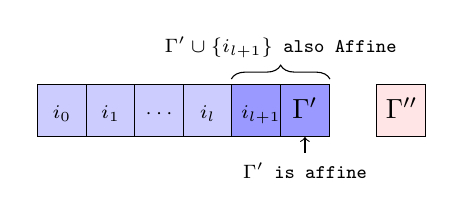
\begin{tikzpicture}[
    font=\ttfamily,
    remember picture,
    array/.style={
      matrix of nodes,
      font=\scriptsize,
      nodes={draw=black, fill=blue!20},
      column sep=-0.5pt,
      row sep=-0.5pt,
      text height=9pt,
      text width =11pt,
      text depth =3pt,
      align=center,
      nodes in empty cells,
      row 1 column 6/.style={font=\normalsize},
      row 1 column 8/.style={font=\normalsize}
      }
    ]

\matrix[array] (A) {
  $i_0$ & $i_1$ & $\cdots$ & $i_{l}$ & |[fill=blue!40]| $i_{l+1}$ & |[fill=blue!40]| $\Gamma'$ & |[draw=none, fill=none]| & |[fill=pink!40]| $\Gamma''$
  \\};

\node [font=\scriptsize\ttfamily,align=center, below=0.2cm of A-1-6.south]  (8) {$\Gamma'$ is affine};

\draw [font=\scriptsize\ttfamily,
  decorate, decoration={brace,amplitude=5pt,raise=.4cm}, xshift=0pt, yshift=-100pt]
    (A-1-5.west) -- (A-1-6.east) node [black,midway,yshift=.8cm] {$\Gamma'\cup\{i_{l+1}\}$ also Affine};

\draw [->] (8.north)--(A-1-6.south);
\end{tikzpicture}
\end{document}
